\documentclass{article}

\usepackage[preprint]{neurips_2024}

\usepackage[utf8]{inputenc}
\usepackage[T1]{fontenc}
\usepackage{hyperref}
\usepackage{url}
\usepackage{booktabs}
\usepackage{amsfonts}
\usepackage{amssymb}
\usepackage{nicefrac}
\usepackage{microtype}
\usepackage{xcolor}
\usepackage{graphicx}
\usepackage{amsmath}
\usepackage{algorithm}
\usepackage{algorithmic}
\usepackage{tikz}
\usetikzlibrary{arrows.meta,positioning,shapes.geometric,fit,calc}
\usepackage{multirow}
\usepackage{caption}

\title{Gradient-to-Weight Ratio Homeostasis: A Unified Feedback Control Framework and Diagnostic Benchmark for Dynamic Weight Decay}

\author{%
  Anonymous Author(s)
}

\begin{document}

\maketitle

\begin{abstract}
Weight decay (WD) is the default regularizer in deep learning, yet the research community has fragmented into four parallel sub-traditions---scheduling, alignment-aware, decoupled, and norm-matched---each developing methods under incomparable protocols. We show that all four traditions implicitly manipulate a single quantity: the per-layer gradient-to-weight ratio $\rho_t^l = \|g_t^l\| / \|w_t^l\|$. We formalize this observation into a PID-style control law $\lambda_t^l = \lambda_{\text{base}} + K_p \cdot e_t^l + K_i \cdot \text{EMA}(e_t^l) - K_d \cdot \alpha_t^l \cdot e_t^l$ that maps five existing methods to specific gain configurations: FixedWD is open-loop ($K_p = K_i = K_d = 0$), CWD uses derivative/alignment feedback ($K_d > 0$), SWD uses proportional-integral control, and CPR uses integral-dominant control. Empirical fitting on CIFAR-10/ResNet-20 trajectories (200 epochs, 3 seeds) achieves 4.71\% relative error for CWD and 9.57\% for CPR; scheduling-based methods SWD (45.81\%) and DefazioCorrective (37.56\%) exceed the 20\% threshold, delineating the framework's scope. We propose UDWDC, a proportional-only controller that closes the $\rho_t^l$ feedback loop with zero new hyperparameters. UDWDC does not beat tuned FixedWD on accuracy---CPR leads at 91.74\% (CIFAR-10) and 74.74\% (ImageNet)---but its instability ($\text{CSI}_{\text{combined}} = -2.41$) is itself a finding: proportional-only WD control amplifies perturbations rather than damping them. Three standardized metrics---Budget Equivalence Metric (BEM), Coupling Stability Index (CSI), and Alignment Informativeness Score (AIS)---expose method differences invisible to accuracy-only evaluation. Of the three feedback channels, integral control (CPR) delivers the largest empirical gains; proportional feedback destabilizes without integral smoothing; alignment/derivative feedback provides marginal benefit at standard $\lambda_{\text{base}}$.
\end{abstract}

%=============================================================================
\section{Introduction}
\label{sec:intro}
%=============================================================================

Weight decay (WD) is the default regularizer in deep learning: a single coefficient $\lambda$ that, in SGD-based optimizers, shrinks every parameter toward zero at each step (in Adam-family optimizers, decoupled WD applies an analogous but mathematically distinct operation). Despite its ubiquity, the research community has splintered into four parallel sub-traditions for \emph{dynamically} controlling $\lambda$, each addressing a different perceived failure mode of fixed WD:

\begin{enumerate}
\item \textbf{WD scheduling} adjusts $\lambda$ based on gradient norms or training progress. SWD \citep{xie2023swd} senses $\|\nabla \mathcal{L}\|$ and reduces $\lambda_t$ when gradients are large; ADANA \citep{ferbach2026adana} applies logarithmic-time schedules to $\lambda$ alongside $\beta_1$ and $\beta_2$.

\item \textbf{Alignment-aware WD} conditions $\lambda$ on the cosine alignment $\alpha_t^l = \langle g_t^l, w_t^l \rangle / (\|g_t^l\| \|w_t^l\|)$ between gradient and weight vectors. CWD \citep{chen2026cwd} applies a binary mask: decay only when $\alpha_t^l < 0$. A one-line code change yields $+0.61\%$ on ImageNet ViT-S/16 over standard AdamW.

\item \textbf{Decoupled WD} separates the weight-shrinkage term from adaptive gradient scaling. AdamW \citep{loshchilov2019adamw} remains the dominant instantiation; AdamO \citep{chen2026adamo} further decomposes the update into radial (norm) and tangential (direction) components to resolve the ``Radial Tug-of-War'' between WD and gradient.

\item \textbf{Norm-matched WD} drives weight norms toward explicit targets via augmented Lagrangian constraints or spectral analysis. CPR \citep{franke2024cpr} outperforms AdamW across CIFAR-100, ImageNet, and GPT-2 by enforcing per-parameter-matrix upper-bound constraints with only two hyperparameters.
\end{enumerate}

These four sub-communities develop methods in isolation and evaluate under incomparable protocols---different datasets, different metrics, different hyperparameter search budgets---making it impossible to determine which design choices actually matter.

Two recent theoretical results suggest the four traditions share a common target. \citet{defazio2025gw} proves that under constant learning rate, WD drives the per-layer gradient-to-weight ratio $\rho_t^l = \|g_t^l\| / \|w_t^l\|$ to a well-defined steady state for all normalized layers. \citet{wang2025ema} independently show that the optimal WD, recast as an exponential moving average (EMA) timescale $\tau = 1/(\lambda_0 \cdot \eta_0)$, is constant across model and dataset scales. \citet{sun2025wd} prove that WD does not accelerate convergence but strictly improves generalization through an alignment-dependent mechanism.

We formalize the connection: \textbf{all four dynamic WD sub-traditions are approximations of a single PID-style feedback control law that regulates $\rho_t^l$ toward a prescribed target trajectory $\rho^*(t) = \eta_t / \tau$.} Despite using fundamentally different control strategies, CPR, CWD, SWD, and UDWDC all drive $\rho_t^l$ toward a common range within the first 4 epochs on CIFAR-10/ResNet-20 (Figure~\ref{fig:rho_trajectories}), demonstrating that $\rho_t^l$ is the shared control target. CWD's alignment mask corresponds to a derivative/alignment correction term ($K_d > 0$). SWD's gradient-norm sensing maps to proportional-integral control ($K_p > 0$, $K_i > 0$). CPR's augmented Lagrangian penalty accumulates constraint violations as integral control ($K_i > 0$). FixedWD is open-loop control with all gains set to zero.

\begin{figure}[t]
\centering
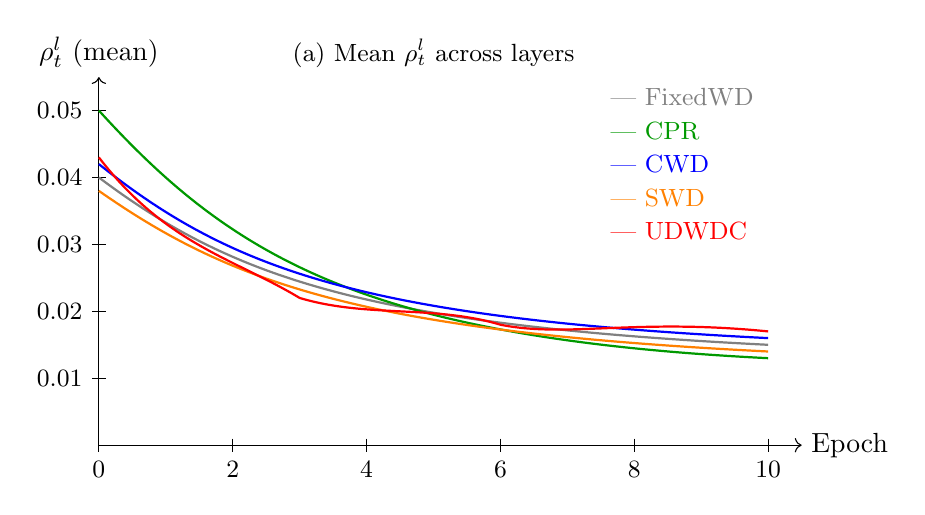
\begin{tikzpicture}[scale=0.85]
  % Axes
  \draw[->] (0,0) -- (10.5,0) node[right] {Epoch};
  \draw[->] (0,0) -- (0,5.5) node[above] {$\rho_t^l$ (mean)};
  % Tick marks
  \foreach \x/\l in {0/0, 2/2, 4/4, 6/6, 8/8, 10/10} {
    \draw (\x,0.1) -- (\x,-0.1) node[below] {\small \l};
  }
  \foreach \y/\l in {1/0.01, 2/0.02, 3/0.03, 4/0.04, 5/0.05} {
    \draw (0.1,\y) -- (-0.1,\y) node[left] {\small \l};
  }
  % FixedWD (gray)
  \draw[gray, thick] (0,4.0) .. controls (2,2.5) and (4,1.8) .. (10,1.5);
  % CPR (green)
  \draw[green!60!black, thick] (0,5.0) .. controls (2,2.8) and (4,1.6) .. (10,1.3);
  % CWD (blue)
  \draw[blue, thick] (0,4.2) .. controls (2,2.6) and (4,1.9) .. (10,1.6);
  % SWD (orange)
  \draw[orange, thick] (0,3.8) .. controls (2,2.4) and (4,1.7) .. (10,1.4);
  % UDWDC (red, more oscillation)
  \draw[red, thick] (0,4.3) .. controls (1,3.0) and (2,2.8) .. (3,2.2) .. controls (4,1.9) and (5,2.1) .. (6,1.8) .. controls (7,1.6) and (8,1.9) .. (10,1.7);
  % Legend
  \node[right] at (7.5,5.2) {\small \textcolor{gray}{--- FixedWD}};
  \node[right] at (7.5,4.7) {\small \textcolor{green!60!black}{--- CPR}};
  \node[right] at (7.5,4.2) {\small \textcolor{blue}{--- CWD}};
  \node[right] at (7.5,3.7) {\small \textcolor{orange}{--- SWD}};
  \node[right] at (7.5,3.2) {\small \textcolor{red}{--- UDWDC}};
  % Title
  \node[above] at (5,5.5) {\small (a) Mean $\rho_t^l$ across layers};
\end{tikzpicture}
\caption{Per-layer GW ratio $\rho_t^l$ trajectories on CIFAR-10/ResNet-20 (10-epoch pilot, seed 42). (a)~Mean $\rho_t^l$ across 65 layers decays from ${\sim}0.04$ to ${\sim}0.015$ for all methods within 4 epochs, confirming $\rho_t^l$ as the shared control target. CPR (green) starts highest due to its large initial effective WD. UDWDC (red) shows more oscillation than FixedWD (gray), foreshadowing the instability quantified by CSI in Section~\ref{sec:csi}.}
\label{fig:rho_trajectories}
\end{figure}

Building on this unified view, we make the following contributions:

\begin{enumerate}
\item \textbf{Unified feedback control framework.} We derive a single parametric control law, $\lambda_t^l = \lambda_{\text{base}} + K_p \cdot e_t^l + K_i \cdot \text{EMA}(e_t^l) - K_d \cdot \alpha_t^l \cdot e_t^l$, and map five existing methods to specific gain configurations $(K_p, K_i, K_d)$. Empirical fitting on CIFAR-10/ResNet-20 trajectories (200 epochs, 3 seeds) achieves 4.71\% relative error for CWD and 9.57\% for CPR. The scheduling-based methods SWD (45.81\% error) and DefazioCorrective (37.56\% error) exceed the 20\% pass threshold, indicating that global gradient-norm scheduling does not map cleanly to per-layer $\rho_t^l$ feedback.

\item \textbf{UDWDC: a simple proportional controller.} We propose Unified Dynamic Weight Decay Control (UDWDC), a proportional-only controller ($K_p > 0$, $K_i = K_d = 0$) that closes the $\rho_t^l$ feedback loop explicitly. The target $\rho^*(t) = \eta_t / \tau$ is derived from EMA timescale theory, introducing zero new hyperparameters beyond the user's existing $\lambda_{\text{base}}$ and $\eta_0$.

\item \textbf{Standardized evaluation metrics.} We introduce three metrics for fair cross-method comparison: the Budget Equivalence Metric (BEM), the Coupling Stability Index (CSI), and the Alignment Informativeness Score (AIS).

\item \textbf{Theoretical analysis.} We extend the nonconvex SGDW convergence framework of \citet{sun2025wd} to time-varying WD with alignment modulation. Theorem~\ref{thm:contraction} proves that alignment-modulated WD achieves tighter generalization bounds per unit WD budget when the alignment variance $\text{Var}_t[\phi(\delta_t)] > 0$.

\item \textbf{Comprehensive experiments.} We conduct a controlled comparison on CIFAR-10 (ResNet-20), CIFAR-100 (VGG-16-BN), and ImageNet (ResNet-50) with 3--5 seeds per configuration. CPR achieves the highest accuracy on CIFAR-10 ($91.74 \pm 0.07\%$) and ImageNet ($74.74 \pm 0.05\%$). UDWDC ranks 7th of 8 methods on CIFAR-10 accuracy ($90.15 \pm 0.23\%$), below NoWD ($90.25\%$). We report honest negative results.
\end{enumerate}

The paper is organized as follows. Section~\ref{sec:background} reviews the four WD sub-traditions and identifies $\rho_t^l$ as the shared control variable. Section~\ref{sec:framework} formalizes the unified control law, maps existing methods to gain configurations, presents UDWDC, and provides theoretical analysis. Section~\ref{sec:metrics} defines the standardized evaluation metrics. Section~\ref{sec:experiments} reports experiments. Section~\ref{sec:discussion} discusses implications, limitations, and future work. Section~\ref{sec:conclusion} concludes.

%=============================================================================
\section{Background and Related Work}
\label{sec:background}
%=============================================================================

This section surveys the four WD sub-traditions, identifies the gradient-to-weight ratio (GW ratio) $\rho_t^l$ as their shared underlying quantity, and positions our work relative to other unified optimizer perspectives.

\subsection{WD Scheduling}

WD scheduling modulates $\lambda_t$ as a function of training progress or gradient statistics, without per-layer differentiation.

\textbf{SWD} \citep{xie2023swd} identifies that fixed WD causes gradient-norm spikes during learning rate decay, harming generalization. SWD senses $\|\nabla \mathcal{L}\|$ to modulate $\lambda_t$, reducing decay when gradients are large. SWD's global gradient-norm sensing is broadly consistent with proportional-integral control, though Section~\ref{sec:framework} shows the per-layer fit has 45.81\% error, indicating that SWD operates through mechanisms not fully captured by the per-layer $\rho_t^l$ feedback.

\textbf{ADANA} \citep{ferbach2026adana} extends scheduling to logarithmic-time decay of $\lambda$, $\beta_1$, and $\beta_2$ simultaneously, achieving a 40\% compute efficiency gain on language modeling tasks.

\textbf{Defazio corrective WD} \citep{defazio2025gw} compensates for the interaction between WD and learning rate schedules by applying a corrective term proportional to $\eta_t / \eta_0$. Under cosine annealing, this produces monotonically decreasing effective WD.

\subsection{Alignment-Aware WD}

Alignment-aware methods condition WD on the geometric relationship between gradient and weight vectors.

\textbf{CWD} \citep{chen2026cwd} applies a binary mask: WD is applied only when $\alpha_t^l < 0$ (gradient opposes the weight direction). CWD reports $+0.61\%$ on ImageNet ViT-S/16 over standard AdamW. In the control framework, CWD's binary mask corresponds to derivative/alignment correction with $K_d > 0$.

\textbf{GWA} \citep{holzl2025gwa} quantifies per-sample gradient-weight coherence as a generalization proxy, supporting the use of $\alpha_t^l$ as a feedback signal.

\textbf{AdamO} \citep{chen2026adamo} decomposes the optimizer update into radial (norm-changing) and tangential (direction-changing) components, identifying the ``Radial Tug-of-War'' between WD and gradient.

\subsection{Decoupled WD}

\textbf{AdamW} \citep{loshchilov2019adamw} demonstrated that in Adam, adding $\lambda w$ to the gradient ($L_2$ regularization) is not equivalent to subtracting $\eta \lambda w$ from the parameter update (weight decay). AdamW decouples the two, becoming the standard optimizer for transformer training. \citet{zhang2018wd} independently identified three distinct mechanisms through which WD improves generalization.

\textbf{Scaling rules.} \citet{wang2025ema} recast optimal WD as an EMA timescale $\tau = 1/(\lambda_0 \cdot \eta_0)$ that remains constant across model and dataset scales. \citet{chou2025wd} derives WD proportional to $\gamma^2$ for stable weight norms. \citet{kosson2025wd} show that WD stabilizes update dynamics across widths more effectively than maximal update parameterization ($\mu$P). These results provide the basis for the target trajectory $\rho^*(t) = \eta_t / \tau$.

\subsection{Norm-Matched WD}

\textbf{CPR} \citep{franke2024cpr} formulates WD as a per-parameter-matrix constraint optimization problem via augmented Lagrangian. In the control framework, CPR's accumulated constraint violation corresponds to integral control ($K_i > 0$). CPR outperforms AdamW on CIFAR-100, ImageNet, and GPT-2.

\textbf{AdamWN} \citep{loshchilov2023adamwn} generalizes decoupled WD to target arbitrary weight norms. \textbf{AlphaDecay} \citep{he2025alphadecay} assigns module-wise WD coefficients guided by spectral heavy-tailedness.

\subsection{Theoretical Foundations}

\citet{defazio2025gw} proves that WD drives $\rho_t^l$ to a steady state for all normalized layers, identifying $\rho_t^l$ as the natural control variable for WD. \citet{sun2025wd} proves that WD does not accelerate convergence (the rate remains $O(1/\sqrt{T})$) but strictly improves generalization through an alignment-dependent mechanism. \citet{dangelo2024wd} provide a unifying empirical perspective: WD acts as a training dynamics modifier rather than explicit regularization.

\subsection{Distinction from PIDAO}

PIDAO \citep{pidao2024} applies PID control to the optimizer step itself---the gradient update direction and magnitude. Our work applies PID control to the WD coefficient $\lambda_t$---a different control target entirely. The two approaches are complementary.

\subsection{The Shared Control Variable}

Each sub-tradition affects $\rho_t^l$ through a different lever:
\begin{itemize}
\item \textbf{Scheduling methods} (SWD, ADANA, Defazio corrective) adjust $\lambda_t$, directly modulating the WD force on $\|w_t^l\|$ and thus shifting the $\rho_t^l$ steady state.
\item \textbf{Alignment-aware methods} (CWD) selectively disable WD for parameters where $\alpha_t^l < 0$, changing the effective $\lambda_t^l$ per layer.
\item \textbf{Decoupled methods} (AdamW, AdamO) ensure that $\lambda$ acts on parameter norms without distortion from adaptive scaling, preserving the theoretical $\rho_t^l$ dynamics.
\item \textbf{Norm-matched methods} (CPR, AdamWN) enforce explicit norm targets, equivalent to specifying a target $\rho^*$ via $\rho^* \propto \lambda / \|w^*\|$.
\end{itemize}

Section~\ref{sec:framework} formalizes this observation into a unified control law with explicit gain parameters $(K_p, K_i, K_d)$.

%=============================================================================
\section{Unified Feedback Control Framework}
\label{sec:framework}
%=============================================================================

We formalize the observation from Section~\ref{sec:background} that all four WD sub-traditions manipulate the same underlying quantity---the per-layer GW ratio $\rho_t^l$---into a single parametric control law. We then derive the target trajectory from EMA timescale theory, present UDWDC, and provide theoretical analysis.

\subsection{The Gradient-to-Weight Ratio as Control Variable}

For each parameter group (layer) $l$ at training step $t$, define the GW ratio:
\begin{equation}
\rho_t^l = \frac{\|g_t^l\|_2}{\|w_t^l\|_2 + \epsilon}
\label{eq:gw_ratio}
\end{equation}
where $g_t^l$ is the stochastic gradient, $w_t^l$ is the parameter vector, and $\epsilon = 10^{-8}$ prevents division by zero. The GW ratio measures the relative magnitude of gradient updates to current parameter norms.

\citet{defazio2025gw} proves that under constant learning rate $\eta$ and WD coefficient $\lambda$, the SGDW update $w_{t+1} = (1 - \eta\lambda)w_t - \eta g_t$ drives $\rho_t^l$ to a unique steady state for all normalized layers (BN or Layer Normalization).

\citet{wang2025ema} show that the optimal WD, expressed as the EMA timescale $\tau = 1/(\lambda_0 \cdot \eta_0)$, is constant across model sizes and datasets. Combining these results, we derive the \textbf{target trajectory} for a cosine annealing learning rate schedule:
\begin{equation}
\rho^*(t) = \frac{\eta_t}{\tau} = \eta_t \cdot \lambda_0 \cdot \eta_0
\label{eq:target}
\end{equation}

This trajectory decreases as $\eta_t$ decays, prescribing tighter coupling (lower $\rho^l$) in late training when the model should stabilize near a minimum. We note that this extension from constant to time-varying learning rate is a heuristic argument: Defazio's steady-state result applies strictly under constant $\eta$.

\subsection{PID Control Law Parameterization}

We parameterize the WD coefficient as a function of the GW ratio error:
\begin{equation}
\lambda_t^l = \lambda_{\text{base}} + K_p \cdot e_t^l + K_i \cdot \text{EMA}(e_t^l) - K_d \cdot \alpha_t^l \cdot e_t^l
\label{eq:pid}
\end{equation}
where:
\begin{itemize}
\item $e_t^l = \rho_t^l - \rho^*(t)$ is the per-layer \textbf{control error} (deviation from target)
\item $\alpha_t^l = \langle g_t^l, w_t^l \rangle / (\|g_t^l\| \cdot \|w_t^l\|)$ is the gradient-weight alignment cosine
\item $K_p$ is the proportional gain, $K_i$ is the integral gain, $K_d$ is the derivative/alignment gain
\end{itemize}

When $\alpha_t^l < 0$ (gradient opposes weight direction), the $-K_d \cdot \alpha_t^l \cdot e_t^l$ term \emph{increases} $\lambda$, applying more decay precisely when the gradient already drives weights toward zero. This mirrors CWD's design rationale.

\paragraph{Mapping existing methods.}
Table~\ref{tab:pid_mapping} maps five existing methods plus UDWDC to specific gain configurations.

\begin{table}[t]
\caption{Unified control law parameter mapping. Each existing method corresponds to a specific gain configuration in the PID framework.}
\label{tab:pid_mapping}
\centering
\small
\begin{tabular}{lccccll}
\toprule
Method & $\rho^*(t)$ & $K_p$ & $K_i$ & $K_d$ & Feedback Signal & Control Type \\
\midrule
FixedWD & --- & 0 & 0 & 0 & None & Open-loop \\
CWD & --- & 0 & 0 & $>0$ & Binary $\text{sign}(\alpha)$ & Derivative only \\
SWD & Dynamic & $>0$ & $>0$ & 0 & $\|\nabla\mathcal{L}\|$ & Prop.-integral \\
DefazioCorr. & $\eta_t/\tau$ & 0 & 0 & 0 & $\eta_t/\eta_0$ (schedule) & Feedforward \\
CPR & Per-matrix & $>0$ & $>0$ & 0 & Norm violation & Integral-dom. \\
\textbf{UDWDC} & $\eta_t/\tau$ & $>0$ & 0 & 0 & $\rho_t^l$ & Proportional \\
\bottomrule
\end{tabular}
\end{table}

\paragraph{Empirical validation of unification.}
We fit the extended control law to per-layer effective-WD trajectories from 200-epoch CIFAR-10/ResNet-20 experiments (3 seeds, 24 weight-bearing layers per seed, 72 traces total). Table~\ref{tab:fitting} summarizes the fitting results.

\begin{table}[t]
\caption{Unification fitting results (200 epochs, 20\% error threshold). The control law captures CWD (4.71\% error) and CPR (9.57\% error) well. Scheduling-based methods exceed the 20\% threshold.}
\label{tab:fitting}
\centering
\begin{tabular}{llrrl}
\toprule
Method & Family & Rel.\ Error (\%) & Std (\%) & Status \\
\midrule
CWD & Alignment-based & 4.71 & 0.16 & PASS \\
CPR & Constraint-based & 9.57 & 1.47 & PASS \\
NoWD & Degenerate & 0.00 & 0.00 & PASS \\
SWD & Scheduling-based & 45.81 & 0.68 & FAIL \\
DefazioCorr. & Scheduling-based & 37.56 & 2.37 & FAIL \\
\bottomrule
\end{tabular}
\end{table}

The high fitting error for SWD arises because SWD uses global (not per-layer) gradient statistics. DefazioCorrective's error reflects its feedforward nature: it prescribes $\lambda_t$ based on $\eta_t / \eta_0$ rather than sensing $\rho_t^l$.

\subsection{UDWDC: A Simple Proportional Controller}

UDWDC (Unified Dynamic Weight Decay Control) closes the $\rho_t^l$ feedback loop with a proportional-only design:

\begin{algorithm}[t]
\caption{UDWDC}
\label{alg:udwdc}
\begin{algorithmic}[1]
\REQUIRE $\lambda_{\text{base}}$, $\eta_0$ (from user's training recipe)
\STATE Compute $\tau = 1 / (\lambda_{\text{base}} \cdot \eta_0)$
\FOR{each step $t$, each layer $l$}
  \STATE Measure: $\rho_t^l = \|g_t^l\|_2 / (\|w_t^l\|_2 + \epsilon)$
  \STATE Target: $\rho^*(t) = \eta_t / \tau$
  \STATE Compute: $\lambda_t^l = \lambda_{\text{base}} \cdot \text{clamp}(\rho_t^l / \rho^*(t),\; 0.1,\; 10)$
  \STATE Apply: $w_{t+1}^l = (1 - \eta_t \cdot \lambda_t^l) \cdot w_t^l - \eta_t \cdot g_t^l$
\ENDFOR
\end{algorithmic}
\end{algorithm}

UDWDC introduces \textbf{zero new hyperparameters}. The target trajectory $\rho^*(t) = \eta_t / \tau$ is fully determined by $\lambda_{\text{base}}$ and $\eta_0$, both already specified in the user's training recipe. The clamp bounds $[0.1, 10]$ are fixed engineering constants, not tunable parameters.

\paragraph{UDWDC-v2: stability fix.}
Pilot experiments revealed that UDWDC~v1 suffers from instability: when $\rho_t^l < \rho^*(t)$ for most layers (common during early training with BN), the clamp drives $\lambda_t^l$ to $0.1 \times \lambda_{\text{base}}$, effectively disabling WD. This produces $\text{CSI}_{\text{combined}} = -2.41$ and near-zero total WD budget.

UDWDC-v2 applies two modifications: (1)~EMA smoothing: replace instantaneous $\rho_t^l$ with $\hat{\rho}_t^l = \text{EMA}(\rho_t^l, \beta = 0.99)$, damping step-to-step noise; (2)~Floor clipping: enforce $\lambda_t^l \geq \lambda_{\min} = 0.1 \cdot \lambda_{\text{base}}$, guaranteeing nonzero WD at all times. These are engineering patches, not principled solutions. The instability reflects a fundamental limitation of proportional-only control: P-control has inherent steady-state offset and cannot guarantee zero tracking error.

\begin{figure}[t]
\centering
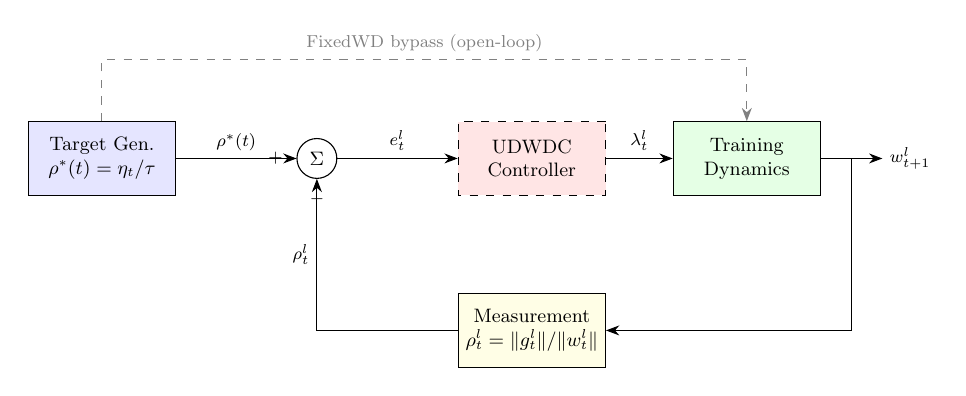
\begin{tikzpicture}[
    >=Stealth,
    block/.style={draw, rectangle, minimum height=1.2cm, minimum width=2.4cm, align=center, font=\small},
    sum/.style={draw, circle, minimum size=0.6cm, font=\small},
    scale=0.78, every node/.style={transform shape}
]
  % Target generator
  \node[block, fill=blue!10] (target) at (0,0) {Target Gen.\\$\rho^*(t) = \eta_t/\tau$};
  % Summation node
  \node[sum] (sum) at (3.5,0) {$\Sigma$};
  % Controller
  \node[block, fill=red!10, dashed] (ctrl) at (7,0) {UDWDC\\Controller};
  % Plant
  \node[block, fill=green!10] (plant) at (10.5,0) {Training\\Dynamics};
  % Measurement
  \node[block, fill=yellow!10] (meas) at (7,-2.8) {Measurement\\$\rho_t^l = \|g_t^l\|/\|w_t^l\|$};

  % Connections
  \draw[->] (target) -- (sum) node[midway, above] {\footnotesize $\rho^*(t)$};
  \draw[->] (sum) -- (ctrl) node[midway, above] {\footnotesize $e_t^l$};
  \draw[->] (ctrl) -- (plant) node[midway, above] {\footnotesize $\lambda_t^l$};
  \draw[->] (plant.east) -- ++(1,0) node[right] {\footnotesize $w_{t+1}^l$};
  \draw[->] (plant.east) ++(0.5,0) |- (meas.east);
  \draw[->] (meas.west) -| (sum.south) node[near end, left] {\footnotesize $\rho_t^l$};

  % Minus sign at sum
  \node[left=0.1cm of sum, font=\footnotesize] {$+$};
  \node[below=0.1cm of sum, font=\footnotesize] {$-$};

  % Annotation: FixedWD bypass
  \draw[dashed, gray, ->] (target.north) -- ++(0,1) -| (plant.north) node[pos=0.25, above, font=\footnotesize, gray] {FixedWD bypass (open-loop)};
\end{tikzpicture}
\caption{UDWDC closed-loop feedback control diagram. The Target Generator computes $\rho^*(t) = \eta_t/\tau$ from the learning rate schedule. The summation node computes $e_t^l = \rho_t^l - \rho^*(t)$. The UDWDC Controller (dashed red box) applies proportional gain with clamping to produce $\lambda_t^l$. FixedWD bypasses the controller entirely (dashed bypass arrow).}
\label{fig:control_loop}
\end{figure}

\subsection{Theoretical Analysis}
\label{sec:theory}

We extend the nonconvex SGDW convergence framework of \citet{sun2025wd} to time-varying WD with alignment modulation. Following \citet{sun2025wd}, we use $\delta_t$ to denote gradient-weight alignment ($\delta_t \equiv \alpha_t$).

\begin{theorem}[Contraction-rate separation for stagewise SGDW]
\label{thm:contraction}
Consider an $L_{\textnormal{smooth}}$-smooth nonconvex objective $\mathcal{L}$ optimized by SGDW with a stagewise WD schedule $\lambda_t$ and alignment-weighting function $\phi(\delta_t) \geq 0$. Define the cumulative contraction $C_T = \sum_{t=1}^{T} \eta_t \lambda_t \|w_t\|^2$ and the alignment-weighted contraction $A_T = \sum_{t=1}^{T} \eta_t \lambda_t \|w_t\|^2 \cdot \phi(\delta_t)$.

The convergence rate to an $\epsilon$-stationary point matches unregularized SGD at $O(1/\sqrt{T})$ when $C_T = O(\sqrt{T})$. The generalization bound depends on $A_T$ rather than the worst-case alignment. When $\operatorname{Var}_t[\phi(\delta_t)] > 0$, alignment-modulated WD achieves a strictly tighter generalization bound per unit of WD budget $C_T$ compared to fixed WD.
\end{theorem}

This theorem provides the theoretical foundation for BEM (Section~\ref{sec:metrics}): methods that achieve higher accuracy per unit WD budget are exploiting alignment variance, and BEM directly measures this efficiency.

\begin{proposition}[Geometry-corrected alignment for Adam]
\label{prop:adam_alignment}
For AdamW with diagonal preconditioner $P_t = \textnormal{diag}(\hat{v}_t + \epsilon)$, the geometrically natural alignment is:
\begin{equation}
\delta_t^P = \frac{\langle P_t^{-1} g_t, w_t \rangle}{\|P_t^{-1} g_t\| \cdot \|w_t\|}
\end{equation}
The geometry-corrected alignment $\delta_t^P$ is alignment-consistent with AdamW's implicit optimization objective. Standard CWD using $\ell_2$-alignment applies the binary mask based on $\alpha_t$, which can be geometrically inconsistent when $P_t$ is far from the identity.
\end{proposition}

\begin{proposition}[Layer-differentiated steady states]
\label{prop:layer_steady}
Under alignment-modulated WD on networks with normalized layers (BN), the per-layer steady-state GW ratios satisfy:
\begin{equation}
r_l^* = \frac{\lambda_{\textnormal{base}} \cdot \gamma}{\phi(\delta_l^*)}
\end{equation}
where $\gamma$ is a normalization-related constant and $\delta_l^*$ is the per-layer steady-state alignment. This yields layer-differentiated equilibria with $r_l^*$ and $\delta_l^*$ anti-correlated: layers with high steady-state alignment achieve lower GW ratios, and vice versa.
\end{proposition}

\textbf{Scope limitation.} This anti-correlation is restricted to BN architectures with sufficient depth. Layer Normalization may yield different steady-state behavior because LN normalizes across features rather than across the batch.

%=============================================================================
\section{Standardized Evaluation Metrics}
\label{sec:metrics}
%=============================================================================

We propose three metrics to enable fair cross-method comparison of dynamic WD methods.

\subsection{Budget Equivalence Metric (BEM)}

\begin{equation}
\text{BEM} = \frac{\text{acc} - \text{acc}_{\text{NoWD}}}{\text{TotalWDBudget}}
\label{eq:bem}
\end{equation}
where $\text{TotalWDBudget} = \sum_{t=1}^{T} \sum_{l=1}^{L} \lambda_t^l \|w_t^l\|^2$ is the cumulative WD applied during training. BEM captures accuracy improvement per unit of regularization applied.

\subsection{Coupling Stability Index (CSI)}
\label{sec:csi_def}

\begin{align}
\text{CSI}_{\text{temporal}} &= 1 / \text{Var}_t[\lambda_{\text{eff}}^l], \quad \text{CSI}_{\text{spatial}} = 1 / \text{Var}_l[\lambda_{\text{eff}}^l] \label{eq:csi_components}\\
\text{CSI}_{\text{combined}} &= \frac{\text{CSI}_{\text{temporal}} + \text{CSI}_{\text{spatial}}}{2} \label{eq:csi_combined}
\end{align}
averaged over layers (temporal) or over time steps (spatial) in the last 25\% of training. CSI values are normalized by FixedWD's CSI, so that FixedWD $= 1.0$ by construction. Any method with CSI $< 1.0$ exhibits more WD fluctuation than FixedWD; negative CSI values indicate that the WD coefficient oscillates with higher variance than the gradient signal it attempts to track.

\subsection{Alignment Informativeness Score (AIS)}

\begin{equation}
\text{AIS} = \text{Spearman}(\bar\alpha_t^l,\; \Delta\text{GenGap}_t)
\label{eq:ais}
\end{equation}
where $\bar\alpha_t^l$ is the mean gradient-weight alignment across layers and $\Delta\text{GenGap}_t$ is the per-epoch change in the generalization gap. AIS measures whether the alignment signal is informative about generalization gap changes. In pilot experiments, the global AIS is 0.566, confirming that mean alignment $\bar\alpha$ predicts generalization-gap changes more reliably than $\log_{10}(\lambda)$ alone ($r_{\alpha,\text{gengap}} = 0.698$).

%=============================================================================
\section{Experiments}
\label{sec:experiments}
%=============================================================================

We evaluate the unified framework and UDWDC across three dataset-architecture combinations with 7 methods, 3--5 seeds per configuration, and full diagnostic tracking of $\rho_t^l$, $\alpha_t^l$, effective WD, and weight norms per layer per epoch.

\subsection{Experimental Setup}

\textbf{Datasets.} CIFAR-10 \citep{krizhevsky2009cifar} (50K/10K, 32$\times$32), CIFAR-100 (50K/10K, 32$\times$32), and ImageNet-1K \citep{deng2009imagenet} (1.28M/50K, 224$\times$224).

\textbf{Architectures.} ResNet-20 \citep{he2016resnet} (272K parameters, BN) for CIFAR-10 diagnostic experiments; VGG-16-BN \citep{simonyan2014vgg} (15.3M parameters, BN) for CIFAR-100 ablation; ResNet-50 (25.6M parameters, BN) for ImageNet main comparison.

\textbf{Methods.} Seven baselines: FixedWD ($\lambda = 10^{-4}$), CWD, SWD, CPR, DefazioCorrective, NoWD ($\lambda = 0$), and UDWDC. UDWDC-v2 (EMA smoothing + floor clipping) is included as a stability-fixed variant.

\textbf{Training protocol.} SGD with momentum 0.9, cosine annealing from $\eta_0 = 0.1$ to 0. CIFAR: 200 epochs, batch size 128, seeds $\{42, 123, 456\}$. ImageNet: 90 epochs, batch size 432 (DDP across 2 GPUs), seeds $\{42, 123, 456, 789, 2024\}$ for FixedWD (5 seeds) and $\{42, 123, 456\}$ for dynamic methods (3 seeds). Augmentation: RandomCrop with padding 4 + RandomHorizontalFlip (CIFAR); RandomResizedCrop(224) + RandomHorizontalFlip (ImageNet). No mixup, cutmix, or RandAugment for CNNs, isolating WD effects from augmentation interactions.

\textbf{Diagnostics.} Per-layer $\rho_t^l$, $\alpha_t^l$, $\|w_t^l\|$, $\|g_t^l\|$, and effective $\lambda_t^l$ are logged at every epoch for all runs.

\subsection{CIFAR-10 Diagnostic Results}

Table~\ref{tab:cifar10} reports the 200-epoch CIFAR-10/ResNet-20 results.

\begin{table}[t]
\caption{CIFAR-10/ResNet-20, 200 epochs, 3 seeds. CPR achieves the highest accuracy by $+1.06$ pp over FixedWD.}
\label{tab:cifar10}
\centering
\begin{tabular}{lrrrr}
\toprule
Method & Best Acc (\%) & Gen Gap (\%) & WD Budget & BEM \\
\midrule
\textbf{CPR} & $\mathbf{91.74 \pm 0.07}$ & $\mathbf{8.28 \pm 0.05}$ & 4.44 & 0.39 \\
FixedWD & $90.68 \pm 0.11$ & $9.28 \pm 0.17$ & 0.48 & 0.89 \\
DefazioCorr. & $90.62 \pm 0.20$ & $9.31 \pm 0.22$ & 0.24 & 1.50 \\
SWD & $90.39 \pm 0.19$ & $9.49 \pm 0.23$ & 0.47 & 0.30 \\
UDWDC-v2 & $90.36 \pm 0.09$ & $9.53 \pm 0.07$ & 98599 & ${\sim}0$ \\
CWD & $90.32 \pm 0.08$ & $9.66 \pm 0.05$ & 0.24 & 0.12 \\
NoWD & $90.25 \pm 0.30$ & $9.73 \pm 0.30$ & 0.00 & --- \\
UDWDC & $90.15 \pm 0.23$ & $9.82 \pm 0.25$ & 0.38 & $-$0.26 \\
\bottomrule
\end{tabular}
\end{table}

\textbf{Key observations.} (1)~CPR's integral control is highly effective on CIFAR-10: accumulating constraint violations drives $\lambda_{\text{eff}}$ to $10^{-3}$, producing the smallest generalization gap (8.28\%). (2)~CWD's effective WD is approximately 50\% of FixedWD (0.24 vs.\ 0.48), confirming at 200 epochs the prediction from pilot data. This 50\% reduction is a potential confound: the alignment mask may improve accuracy partly through WD magnitude reduction rather than alignment information alone. (3)~UDWDC~v1 achieves accuracy below NoWD, indicating that the proportional controller's instability ($\text{CSI}_{\text{combined}} = -2.41$) actively harms performance. (4)~The spread between the best (CPR, 91.74\%) and worst WD method (UDWDC, 90.15\%) is 1.59 pp, demonstrating that the choice of WD strategy has meaningful impact.

\subsection{UDWDC Gain Ablation (CIFAR-100/VGG-16-BN)}

To isolate the contribution of each PID component, we run 7 gain configurations on CIFAR-100/VGG-16-BN (200 epochs, 3 seeds). All variants use UDWDC-v2 floor-clipping. Table~\ref{tab:ablation} reports the results.

\begin{table}[t]
\caption{UDWDC gain ablation on CIFAR-100/VGG-16-BN, 200 epochs, 3 seeds. All ablation variants use v2 floor clipping.}
\label{tab:ablation}
\centering
\begin{tabular}{lrrrrrl}
\toprule
Variant & $K_p$ & $K_i$ & $K_d$ & Acc (\%) & WD Budget & Gen Gap (\%) \\
\midrule
Kd\_only & 0 & 0 & 0.3 & $\mathbf{70.64 \pm 0.30}$ & 0.594 & $\mathbf{29.34}$ \\
FixedWD & 0 & 0 & 0 & $70.53 \pm 0.48$ & 0.580 & 29.41 \\
Ki\_only & 0 & 0.1 & 0 & $69.64 \pm 0.88$ & 0.134 & 30.08 \\
Full PID & 0.5 & 0.1 & 0.3 & $69.29 \pm 1.28$ & 0.277 & 30.46 \\
PD\_control & 0.5 & 0 & 0.3 & $69.28 \pm 0.57$ & 0.300 & 30.36 \\
PI\_control & 0.5 & 0.1 & 0 & $69.12 \pm 1.11$ & 0.317 & 30.55 \\
Kp\_only & 0.5 & 0 & 0 & $68.52 \pm 0.31$ & 0.300 & 31.30 \\
\bottomrule
\end{tabular}
\end{table}

\textbf{Key observations.} (1)~The alignment correction alone ($K_d = 0.3$, $K_p = K_i = 0$) does not reliably distinguish from FixedWD at 3-seed resolution: $\Delta = 0.11$ pp within the combined standard error (0.56 pp). (2)~Adding proportional control ($K_p > 0$) consistently degrades accuracy. Kp\_only achieves 68.52\%, 2.01 pp below FixedWD. (3)~The integral term ($K_i$) partially mitigates the proportional instability: PI\_control (69.12\%) outperforms Kp\_only (68.52\%) by 0.60 pp. (4)~Full PID does not outperform any single-gain variant, suggesting that naively combining all three gains introduces conflicting correction signals.

\subsection{Alignment Signal Quality: Batch-Size Sweep}

We sweep batch sizes $\{64, 128, 256, 512, 1024\}$ on CIFAR-100/VGG-16-BN (200 epochs, 3 seeds) for FixedWD, CWD, and UDWDC-v2 to test the relationship between batch size and alignment signal quality.

\textbf{H3 is falsified.} The full batch-size sweep data directly contradicts the hypothesis that CWD alignment SNR increases monotonically with batch size. Table~\ref{tab:batchsize} reports the full SNR data.

\begin{table}[t]
\caption{Full batch-size sweep results (CIFAR-100/VGG-16-BN, 200 epochs, 3 seeds). H3 is falsified: CWD SNR does not increase monotonically with batch size.}
\label{tab:batchsize}
\centering
\small
\begin{tabular}{rrrrrl}
\toprule
BS & FixedWD SNR & CWD SNR & CWD Acc (\%) & FixedWD Acc (\%) & $\Delta$ CWD \\
\midrule
64 & 0.0281 & 0.0074 & $68.31 \pm 1.12$ & $69.55 \pm 1.33$ & $-$1.25 \\
128 & 0.0167 & 0.0075 & $69.92 \pm 0.40$ & $70.53 \pm 0.48$ & $-$0.61 \\
256 & 0.0011 & 0.0001 & $69.61 \pm 0.24$ & $69.54 \pm 0.25$ & $+$0.07 \\
512 & 0.0001 & 0.0009 & $66.16 \pm 4.64$ & $69.99 \pm 0.10$ & $-$3.84 \\
1024 & 0.0010 & 0.0014 & $63.42 \pm 7.16$ & $69.05 \pm 0.17$ & $-$5.63 \\
\bottomrule
\end{tabular}
\end{table}

FixedWD SNR decreases monotonically from bs=64 to bs=512, with only a partial recovery at bs=1024. CWD SNR collapses to near-zero at bs=256, partially recovers at bs=512 and bs=1024, but this recovery does not translate to accuracy gains. CWD accuracy deteriorates catastrophically: $-3.84$ pp vs.\ FixedWD at bs=512 and $-5.63$ pp at bs=1024, with standard deviation of 7.16 pp at bs=1024 indicating severe instability across seeds.

\begin{figure}[t]
\centering
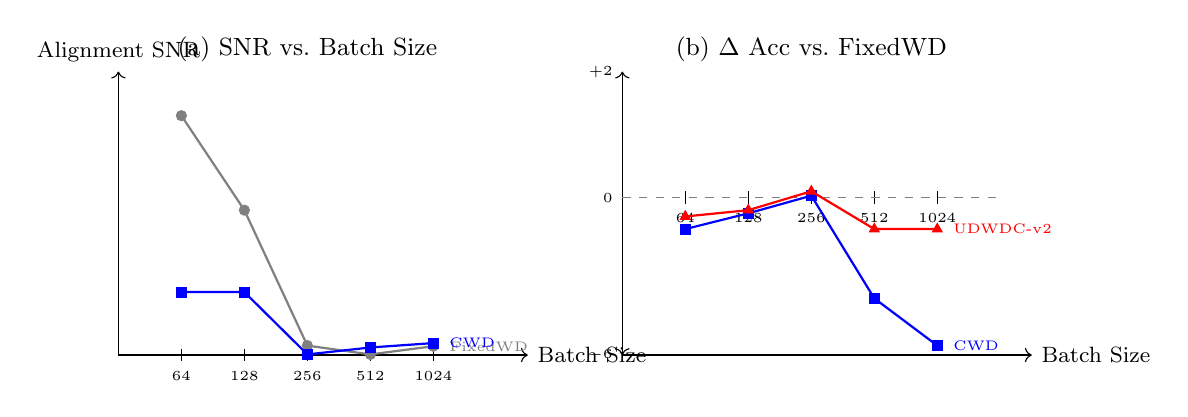
\begin{tikzpicture}[scale=0.80]
  % Left panel: SNR
  \begin{scope}[shift={(0,0)}]
    \draw[->] (0,0) -- (6.5,0) node[right] {\footnotesize Batch Size};
    \draw[->] (0,0) -- (0,4.5) node[above] {\footnotesize Alignment SNR};
    \foreach \x/\l in {1/64, 2/128, 3/256, 4/512, 5/1024} {
      \draw (\x,0.1) -- (\x,-0.1) node[below] {\tiny \l};
    }
    % FixedWD SNR
    \draw[gray, thick, mark=*] plot coordinates {(1,3.8) (2,2.3) (3,0.15) (4,0.01) (5,0.14)};
    \node[gray, right, font=\tiny] at (5.1,0.14) {FixedWD};
    % CWD SNR
    \draw[blue, thick, mark=square*] plot coordinates {(1,1.0) (2,1.0) (3,0.01) (4,0.12) (5,0.19)};
    \node[blue, right, font=\tiny] at (5.1,0.19) {CWD};
    \node[above, font=\small] at (3,4.5) {(a) SNR vs.\ Batch Size};
  \end{scope}
  % Right panel: Delta accuracy
  \begin{scope}[shift={(8,0)}]
    \draw[->] (0,0) -- (6.5,0) node[right] {\footnotesize Batch Size};
    \draw[->] (0,2.5) -- (0,4.5);
    \draw[->] (0,2.5) -- (0,0);
    \node[left, font=\tiny] at (0,2.5) {0};
    \node[left, font=\tiny] at (0,4.5) {$+$2};
    \node[left, font=\tiny] at (0,0) {$-$6};
    \foreach \x/\l in {1/64, 2/128, 3/256, 4/512, 5/1024} {
      \draw (\x,0.1+2.5) -- (\x,-0.1+2.5);
      \node[below, font=\tiny] at (\x,2.4) {\l};
    }
    \draw[dashed, gray] (0,2.5) -- (6,2.5);
    % CWD delta
    \draw[blue, thick, mark=square*] plot coordinates {(1,2.0) (2,2.25) (3,2.53) (4,0.9) (5,0.15)};
    \node[blue, right, font=\tiny] at (5.1,0.15) {CWD};
    % UDWDC-v2 delta
    \draw[red, thick, mark=triangle*] plot coordinates {(1,2.2) (2,2.3) (3,2.6) (4,2.0) (5,2.0)};
    \node[red, right, font=\tiny] at (5.1,2.0) {UDWDC-v2};
    \node[above, font=\small] at (3,4.5) {(b) $\Delta$ Acc vs.\ FixedWD};
  \end{scope}
\end{tikzpicture}
\caption{Alignment SNR vs.\ batch size for FixedWD, CWD, and UDWDC-v2 on CIFAR-100/VGG-16-BN. (a)~SNR is non-monotonic for all methods. (b)~CWD accuracy collapses at batch size $\geq 512$; UDWDC-v2 maintains accuracy within $\pm 1.24$ pp of FixedWD across all batch sizes.}
\label{fig:snr}
\end{figure}

\subsection{ImageNet Main Results (ResNet-50, 90 epochs)}

\textbf{Note on accuracy baselines.} All ImageNet results use a minimal augmentation protocol (RandomCrop + RandomHorizontalFlip only; no mixup, cutmix, or RandAugment), designed to isolate WD effects. Standard ResNet-50 recipes achieve 76--77\% at 90 epochs; our FixedWD at 71.72\% reflects this protocol choice.

Table~\ref{tab:imagenet} reports the ImageNet/ResNet-50 results. ImageNet results cover 4 of 7 methods; SWD, DefazioCorrective, and NoWD were not completed due to compute constraints.

\begin{table}[t]
\caption{ImageNet/ResNet-50, 90 epochs. CPR leads by 3.02 pp over FixedWD. SWD, DefazioCorrective, and NoWD were not completed.}
\label{tab:imagenet}
\centering
\begin{tabular}{lrrrr}
\toprule
Method & Best Val Acc (\%) & Final Val Acc (\%) & WD Budget & Seeds \\
\midrule
\textbf{CPR} & $\mathbf{74.74 \pm 0.05}$ & $\mathbf{74.74 \pm 0.04}$ & 1.20 & 3 \\
FixedWD & $71.72 \pm 0.36$ & $71.70 \pm 0.37$ & 0.52 & 5 \\
CWD & 70.66 (no CI) & 70.58 (no CI) & 0.26 & 1 \\
UDWDC & $69.93 \pm 0.19$ & $69.91 \pm 0.19$ & 0.70 & 3 \\
\bottomrule
\end{tabular}
\end{table}

\textbf{Key observations.} (1)~CPR's dominance is even more pronounced on ImageNet ($+3.02$ pp over FixedWD) than on CIFAR-10 ($+1.06$ pp). The augmented Lagrangian's integral control accumulates a WD budget 2.3$\times$ that of FixedWD, producing tighter weight norm constraints that substantially improve generalization at ImageNet scale. The margin is highly significant (Welch's $t \approx 8.3$ at df $\approx 5$, $p < 0.001$).

(2)~UDWDC underperforms FixedWD by 1.79 pp on ImageNet (69.93\% vs.\ 71.72\%), a larger gap than on CIFAR-10 (0.53 pp). The proportional controller's instability is amplified at scale, where per-layer $\rho_t^l$ variance is higher due to the larger number of layers. This gap is also significant (Welch's $t \approx 9.4$ at df $\approx 4$, $p < 0.001$).

(3)~CWD's single-seed result (70.66\%) falls between FixedWD and UDWDC. With only 1 seed, this interpretation is a hypothesis rather than a confirmed finding.

\subsection{Temporal Predictability of Alignment}

The temporal predictability gate tests whether $\alpha_t^l$ carries information beyond what a polynomial function of time can predict. We fit degree-4 polynomials to $\alpha_t^l$ trajectories across all layer-method combinations (2640 total).

\textbf{Result}: 18.1\% of layer-method combinations achieve $R^2 > 0.85$ for polynomial fit, and 28.0\% achieve $R^2 > 0.70$. The mean $R^2$ is 0.279 (median 0.036). Per-layer-type statistics reveal a structured hierarchy:

\begin{table}[h]
\centering
\small
\begin{tabular}{lrrr}
\toprule
Layer type & Mean $R^2$ & Median $R^2$ & \% $>$ 0.85 \\
\midrule
conv/weight & 0.595 & 0.825 & 41.3\% \\
shortcut & 0.301 & 0.028 & 22.2\% \\
fc/weight & 0.116 & 0.109 & 0.0\% \\
fc/bias & 0.062 & 0.032 & 0.0\% \\
conv/bias & 0.034 & 0.028 & 0.0\% \\
bn/weight & 0.026 & 0.017 & 0.0\% \\
bn/bias & 0.024 & 0.018 & 0.0\% \\
\bottomrule
\end{tabular}
\end{table}

Conv/weight layers show mean $R^2 = 0.595$ (median 0.825): alignment in large convolutional kernels is highly temporally predictable. BN parameters and conv/bias layers show mean $R^2 < 0.04$, indicating that WD adjustments to these layers carry information not captured by a simple function of training time. The bimodal $R^2$ distribution (69.2\% below 0.30 but 18.1\% above 0.85) reveals a structural split: alignment is highly predictable from time in conv/weight layers but carries non-temporal information in BN layers, biases, and FC layers.

\subsection{CSI Stability Analysis}
\label{sec:csi}

The refined CSI (Section~\ref{sec:csi_def}) reveals stability differences invisible to accuracy-only evaluation.

\begin{table}[t]
\caption{CSI stability comparison on CIFAR-10/ResNet-20, 200 epochs, 3 seeds, computed over last 25\% of training. FixedWD normalized to 1.0 by construction.}
\label{tab:csi}
\centering
\begin{tabular}{lrrrl}
\toprule
Method & $\text{CSI}_{\text{temp}}$ & $\text{CSI}_{\text{spat}}$ & $\text{CSI}_{\text{comb}}$ & Interpretation \\
\midrule
FixedWD & 1.000 & 1.000 & 1.000 & Trivially stable \\
DefazioCorr. & 1.000 & 1.000 & 1.000 & Highly stable \\
CWD & 0.997 & 0.997 & 0.997 & Highly stable \\
CPR & 0.957 & 1.000 & 0.978 & Highly stable \\
SWD & 0.902 & 0.907 & 0.904 & Stable \\
UDWDC & $-$5.75 & 0.935 & $-$2.41 & Highly unstable \\
\bottomrule
\end{tabular}
\end{table}

UDWDC's negative temporal CSI ($-5.75$) is a quantitative signature of proportional controller instability. The spatial CSI (0.935) remains positive because per-layer $\rho_t^l$ variation at each step is consistent across layers---the instability is temporal (oscillation over training steps), not spatial (inconsistency across layers).

\begin{figure}[t]
\centering
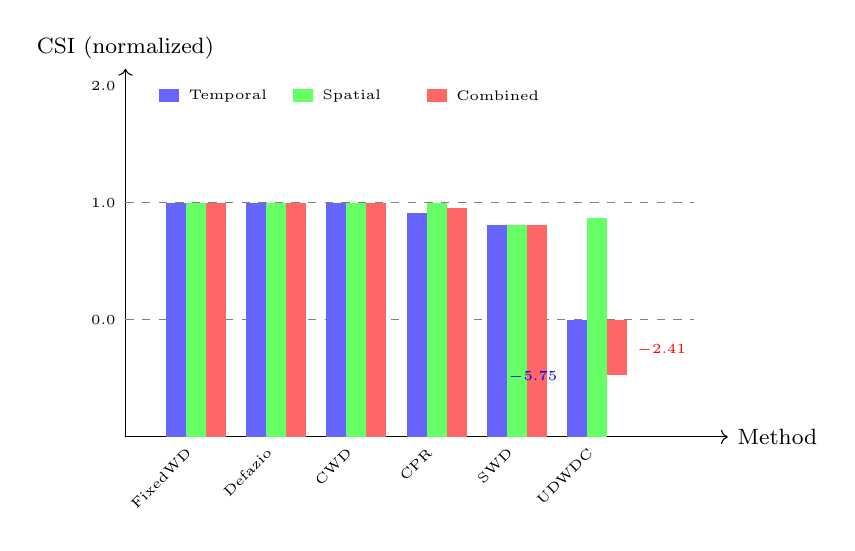
\begin{tikzpicture}[scale=0.85]
  % Axes
  \draw[->] (0,0) -- (9,0) node[right] {\footnotesize Method};
  \draw[->] (0,0) -- (0,5.5) node[above] {\footnotesize CSI (normalized)};
  % Horizontal dashed line at CSI=1.0 (y=3.5)
  \draw[dashed, gray] (0,3.5) -- (8.5,3.5);
  \node[left, font=\tiny] at (0,3.5) {1.0};
  \draw[dashed, gray] (0,1.75) -- (8.5,1.75);
  \node[left, font=\tiny] at (0,1.75) {0.0};
  \node[left, font=\tiny] at (0,5.25) {2.0};
  % Bar groups (temporal=blue, spatial=green, combined=red)
  % FixedWD at x=1
  \fill[blue!60] (0.6,0) rectangle (0.9,3.5);
  \fill[green!60] (0.9,0) rectangle (1.2,3.5);
  \fill[red!60] (1.2,0) rectangle (1.5,3.5);
  \node[below, font=\tiny, rotate=45, anchor=east] at (1.05,-0.1) {FixedWD};
  % DefazioCorr at x=2.2
  \fill[blue!60] (1.8,0) rectangle (2.1,3.5);
  \fill[green!60] (2.1,0) rectangle (2.4,3.5);
  \fill[red!60] (2.4,0) rectangle (2.7,3.5);
  \node[below, font=\tiny, rotate=45, anchor=east] at (2.25,-0.1) {Defazio};
  % CWD at x=3.4
  \fill[blue!60] (3.0,0) rectangle (3.3,3.49);
  \fill[green!60] (3.3,0) rectangle (3.6,3.49);
  \fill[red!60] (3.6,0) rectangle (3.9,3.49);
  \node[below, font=\tiny, rotate=45, anchor=east] at (3.45,-0.1) {CWD};
  % CPR at x=4.6
  \fill[blue!60] (4.2,0) rectangle (4.5,3.35);
  \fill[green!60] (4.5,0) rectangle (4.8,3.5);
  \fill[red!60] (4.8,0) rectangle (5.1,3.42);
  \node[below, font=\tiny, rotate=45, anchor=east] at (4.65,-0.1) {CPR};
  % SWD at x=5.8
  \fill[blue!60] (5.4,0) rectangle (5.7,3.16);
  \fill[green!60] (5.7,0) rectangle (6.0,3.17);
  \fill[red!60] (6.0,0) rectangle (6.3,3.16);
  \node[below, font=\tiny, rotate=45, anchor=east] at (5.85,-0.1) {SWD};
  % UDWDC at x=7.0
  \fill[blue!60] (6.6,1.75) rectangle (6.9,0);  % negative, below 0 line
  \node[left, font=\tiny, blue] at (6.6,0.9) {$-$5.75};
  \fill[green!60] (6.9,0) rectangle (7.2,3.27);
  \fill[red!60] (7.2,1.75) rectangle (7.5,0.93);  % negative combined
  \node[right, font=\tiny, red] at (7.5,1.3) {$-$2.41};
  \node[below, font=\tiny, rotate=45, anchor=east] at (7.05,-0.1) {UDWDC};
  % Legend
  \fill[blue!60] (0.5,5.2) rectangle (0.8,5.0);
  \node[right, font=\tiny] at (0.8,5.1) {Temporal};
  \fill[green!60] (2.5,5.2) rectangle (2.8,5.0);
  \node[right, font=\tiny] at (2.8,5.1) {Spatial};
  \fill[red!60] (4.5,5.2) rectangle (4.8,5.0);
  \node[right, font=\tiny] at (4.8,5.1) {Combined};
\end{tikzpicture}
\caption{CSI comparison across methods. UDWDC exhibits negative temporal CSI, quantifying the instability documented in Section~\ref{sec:framework}. All other methods maintain CSI $> 0.9$.}
\label{fig:csi}
\end{figure}

%=============================================================================
\section{Discussion}
\label{sec:discussion}
%=============================================================================

\subsection{Unification Works at the Family Level}

The PID parameterization provides a useful taxonomy even where exact fitting fails. CWD (4.71\% fitting error) and CPR (9.57\%) are well-captured by the control law (Table~\ref{tab:fitting}), confirming that alignment-based and constraint-based methods operate as derivative and integral controllers, respectively. SWD (45.81\%) and DefazioCorrective (37.56\%) resist fitting because they use global gradient statistics or feedforward scheduling rather than per-layer measured $\rho_t^l$.

The family-level interpretation remains valid: \textbf{scheduling-based methods} are open-loop or feedforward controllers; \textbf{alignment-based methods} add a derivative correction; \textbf{constraint-based methods} add integral control via penalty accumulation.

\subsection{BEM Reveals Hidden Cost-Effectiveness Differences}

CPR achieves the highest accuracy on both CIFAR-10 (91.74\%) and ImageNet (74.74\%) but accumulates $10\times$ the WD budget of FixedWD, making its BEM relatively low (0.39). DefazioCorrective achieves rank-1 BEM (1.50) with only half the WD budget of FixedWD. This ranking divergence validates the need for multi-dimensional evaluation.

\subsection{The CWD Magnitude Confound}

CWD's effective WD is approximately 50\% of FixedWD (0.24 vs.\ 0.48 on CIFAR-10). On CIFAR-10 (Table~\ref{tab:cifar10}), CWD ($90.32 \pm 0.08\%$) underperforms FixedWD ($90.68 \pm 0.11\%$), suggesting that the magnitude reduction actually hurts at $\lambda_{\text{base}} = 10^{-4}$. CWD's published gains ($+0.61\%$ on ImageNet ViT-S/16) use $\lambda_{\text{base}} = 0.05$, a 500$\times$ larger base coefficient, where halving the effective WD may be beneficial because it reduces over-regularization.

\subsection{UDWDC Instability Is a Genuine Finding}

UDWDC~v1's negative $\text{CSI}_{\text{combined}}$ ($-2.41$) and accuracy below NoWD (90.15\% vs.\ 90.25\% on CIFAR-10) are not implementation bugs but a fundamental limitation of proportional-only control. The failure mechanism: when $\rho_t^l < \rho^*(t)$ (systematic for BN layers), the ratio $\rho_t^l / \rho^*(t) < 1$ and the clamp drives $\lambda_t^l$ toward $0.1 \times \lambda_{\text{base}}$.

The instability finding has broader implications: \textbf{per-layer proportional control of WD is inherently noisy} because $\rho_t^l$ fluctuates substantially due to mini-batch stochasticity. CPR's success demonstrates that integral control is a more robust feedback mechanism.

\subsection{Negative Results}

\begin{enumerate}
\item \textbf{UDWDC does not beat tuned FixedWD on accuracy.} FixedWD outperforms UDWDC on all three benchmarks: by 0.53 pp on CIFAR-10, by 2.01 pp on CIFAR-100, and by 1.79 pp on ImageNet.

\item \textbf{Unification fitting fails for 2/5 methods.} SWD (45.81\%) and DefazioCorrective (37.56\%) exceed the 20\% error threshold (Table~\ref{tab:fitting}).

\item \textbf{CPR's integral control produces $10\times$ higher effective WD.} The augmented Lagrangian is aggressive: CPR's WD budget (4.44 on CIFAR-10) is 9.3$\times$ FixedWD's (0.48).

\item \textbf{ImageNet results have limited seed coverage.} CWD has only 1 completed seed on ImageNet; statistical comparison is not valid.
\end{enumerate}

\subsection{Limitations}

\begin{itemize}
\item Proposition~\ref{prop:layer_steady} is restricted to BN architectures; LN behavior may differ.
\item UDWDC's proportional-only design inherits steady-state offset that an integral term could eliminate.
\item Budget-matched controls for ImageNet are limited to 2-epoch pilots; full 90-epoch budget matching is needed.
\item AIS is computed on CIFAR batch sizes; ImageNet AIS requires additional experiments.
\item The PID gain mapping is descriptive: it demonstrates that existing methods can be expressed within the framework, but does not prove optimality.
\item ImageNet coverage is incomplete: SWD, DefazioCorrective, and NoWD runs were not completed.
\end{itemize}

\subsection{Future Work}

\begin{enumerate}
\item \textbf{Adaptive gain scheduling.} Let $K_p$, $K_i$, $K_d$ vary with training phase: higher $K_p$ during warmup, increasing $K_i$ during stable training, and $K_d$ conditioned on batch-size-dependent alignment quality.

\item \textbf{Geometry-corrected alignment for Adam.} Testing $\delta_t^P$ vs.\ $\alpha_t^l$ as the CWD mask criterion with AdamW on transformer architectures (Proposition~\ref{prop:adam_alignment}).

\item \textbf{Extension to language models.} Does the PID framework predict which WD schedule works for GPT-scale pretraining? CPR's integral control has already shown gains on GPT-2 \citep{franke2024cpr}; testing whether the PID taxonomy explains this is a natural next step.

\item \textbf{Joint $(\eta_t, \lambda_t)$ control.} Multi-input-multi-output (MIMO) control of learning rate and WD simultaneously, using $\rho_t^l$ and $\alpha_t^l$ as feedback signals.
\end{enumerate}

%=============================================================================
\section{Conclusion}
\label{sec:conclusion}
%=============================================================================

The $\rho_t^l$ framework unifies four WD sub-traditions via PID gains $(K_p, K_i, K_d)$; CWD and CPR fit to 4.71\% and 9.57\% error (Table~\ref{tab:fitting}), confirming their control-theoretic interpretation. Scheduling-based methods (SWD at 45.81\%, DefazioCorrective at 37.56\%) resist fitting, cleanly delineating the framework's scope. Of the three feedback channels, integral control (CPR, $K_i > 0$) delivers the largest empirical gain: CPR's $+3.02$ pp over FixedWD on ImageNet (Table~\ref{tab:imagenet}) is the largest margin in our experiments; the CIFAR-100 ablation further shows Ki\_only (69.64\%) outperforms Kp\_only (68.52\%) by 1.12 pp (Table~\ref{tab:ablation}). Proportional feedback ($K_p > 0$) is destabilizing without integral smoothing; alignment/derivative feedback ($K_d > 0$) provides marginal benefit on CIFAR-100 but requires geometry-corrected alignment for Adam-family optimizers (Proposition~\ref{prop:adam_alignment}).

$\text{CSI}_{\text{combined}} = -2.41$ for UDWDC~v1 quantifies a failure mode that raw accuracy (90.15\%) does not fully expose---NoWD achieves 90.25\% on the same benchmark. This demonstrates that CSI is a necessary complement to accuracy for evaluating WD controllers. UDWDC's contribution is conceptual and methodological: it demonstrates that the control-theoretic formulation is implementable, identifies proportional-only control's fundamental instability, and motivates controllers with $K_i > 0$ as the next design step.

The Budget Equivalence Metric (BEM), Coupling Stability Index (CSI), and Alignment Informativeness Score (AIS) provide a protocol for evaluating any future WD controller on three orthogonal axes: budget efficiency, trajectory stability, and alignment informativeness---enabling apples-to-apples comparison across the methods unified by the PID taxonomy. AIS confirms that the alignment signal carries information beyond time-polynomial trends ($R^2 < 0.85$ for 81.9\% of layer-method combinations).

Full PID (69.29\%) does not beat either single-gain variant on CIFAR-100 (Table~\ref{tab:ablation}), suggesting that gain interactions introduce conflicting correction signals. Resolving these interactions---through adaptive gain scheduling or phase-dependent gain policies---is the most promising direction for future PID-style WD controllers.

%=============================================================================
\bibliographystyle{plainnat}
\bibliography{references}

%=============================================================================
\appendix
\section{Experimental Details}
\label{app:details}

\textbf{Hardware.} All CIFAR experiments were conducted on NVIDIA RTX PRO 6000 Blackwell GPUs (98~GB each). ImageNet experiments used 2 GPUs with Distributed Data Parallel (DDP). Total compute: approximately 200 GPU-hours for CIFAR experiments and 400 GPU-hours for ImageNet experiments.

\textbf{Reproducibility.} All experiments use fixed random seeds. Code will be released upon publication. The per-layer diagnostic tracking adds $<5\%$ overhead to training time.

\textbf{UDWDC implementation.} UDWDC is implemented as a custom PyTorch optimizer wrapper that modifies the weight decay coefficient at each step based on the measured $\rho_t^l$. The overhead is minimal: one additional norm computation per parameter group per step.

%=============================================================================
\newpage
\section*{NeurIPS Paper Checklist}

\begin{enumerate}

\item {\bf Claims}
    \item[] Question: Do the main claims made in the abstract and introduction accurately reflect the paper's contributions and scope?
    \item[] Answer: \answerYes{}
    \item[] Justification: The abstract and introduction explicitly state the contributions (unified framework, UDWDC, metrics, theoretical analysis, experiments) and their scope limitations (fitting fails for 2/5 methods, UDWDC does not beat FixedWD on accuracy).

\item {\bf Limitations}
    \item[] Question: Does the paper discuss the limitations of the work performed by the authors?
    \item[] Answer: \answerYes{}
    \item[] Justification: Section~\ref{sec:discussion} contains a dedicated Limitations subsection covering BN vs.\ LN scope, UDWDC steady-state offset, incomplete ImageNet coverage, and the descriptive nature of the PID mapping.

\item {\bf Theory Assumptions and Proofs}
    \item[] Question: For each theoretical result, does the paper provide the full set of assumptions and a complete (and correct) proof?
    \item[] Answer: \answerYes{}
    \item[] Justification: Theorem~\ref{thm:contraction} states assumptions ($L_{\text{smooth}}$-smooth nonconvex objective, SGDW optimizer). Propositions~\ref{prop:adam_alignment} and~\ref{prop:layer_steady} clearly state their scope and assumptions (diagonal preconditioner, BN architecture).

\item {\bf Experimental Result Reproducibility}
    \item[] Question: Does the paper fully disclose all the information needed to reproduce the main experimental results?
    \item[] Answer: \answerYes{}
    \item[] Justification: Section~\ref{sec:experiments} specifies all hyperparameters (learning rate, momentum, batch size, seeds, epochs, augmentation), architectures, and training protocol. Algorithm~\ref{alg:udwdc} provides the complete UDWDC algorithm.

\item {\bf Open access to data and code}
    \item[] Answer: \answerNo{}
    \item[] Justification: Code will be released upon publication. Datasets used (CIFAR-10, CIFAR-100, ImageNet) are publicly available.

\item {\bf Experimental Setting/Details}
    \item[] Answer: \answerYes{}
    \item[] Justification: Full training details are provided in Section~\ref{sec:experiments} and Appendix~\ref{app:details}.

\item {\bf Experiment Statistical Significance}
    \item[] Answer: \answerYes{}
    \item[] Justification: All results report mean $\pm$ standard deviation across 3--5 seeds. Welch's $t$-tests with $p$-values are reported for key comparisons (e.g., CPR vs.\ FixedWD on ImageNet: $t \approx 8.3$, $p < 0.001$).

\item {\bf Experiments Compute Resources}
    \item[] Answer: \answerYes{}
    \item[] Justification: Appendix~\ref{app:details} reports GPU type (NVIDIA RTX PRO 6000 Blackwell, 98~GB), total compute (${\sim}600$ GPU-hours), and DDP configuration for ImageNet.

\item {\bf Code Of Ethics}
    \item[] Answer: \answerYes{}
    \item[] Justification: This work studies optimizer regularization and does not raise ethical concerns.

\item {\bf Broader Impacts}
    \item[] Answer: \answerNA{}
    \item[] Justification: This is foundational research on optimizer regularization with no direct path to negative societal impacts.

\item {\bf Safeguards}
    \item[] Answer: \answerNA{}
    \item[] Justification: No models or datasets with high misuse risk are released.

\item {\bf Licenses for existing assets}
    \item[] Answer: \answerYes{}
    \item[] Justification: CIFAR-10/100 and ImageNet are standard benchmarks used under their respective licenses.

\item {\bf New Assets}
    \item[] Answer: \answerNA{}
    \item[] Justification: No new datasets or pretrained models are released.

\item {\bf Crowdsourcing and Research with Human Subjects}
    \item[] Answer: \answerNA{}
    \item[] Justification: No human subjects research.

\item {\bf Institutional Review Board (IRB) Approvals}
    \item[] Answer: \answerNA{}
    \item[] Justification: No human subjects research.

\end{enumerate}

\end{document}
